\documentclass[10pt,a4paper]{article}
\usepackage{fontspec,polyglossia}
\setmainlanguage{russian}
\setmainfont{Times New Roman}
\usepackage{amsmath,amssymb,booktabs,tabularx,graphicx}
\usepackage[margin=17mm]{geometry}
\usepackage[hidelinks]{hyperref}
\usepackage{titlesec}
\titleformat{\section}{\large\bfseries}{}{0pt}{}
\titlespacing*{\section}{0pt}{8pt}{4pt}
\setlength{\parindent}{0pt}
\setlength{\parskip}{4pt}
\setlength{\emergencystretch}{3em}
\begin{document}
{\Large\bfseries MG как триггер диагностики при циклическом обучении текстового VAE}\par\medskip

29 сентября 2026. Пилот 100; девять новых инициализаций 101--109. Код и настройки предыдущих экспериментов сохранены.

\textbf{Главный результат.} Практическое преимущество выбранного MG-монитора в основном сравнении не подтверждено. MG обнаружил меньше событий, чем проверки через равные интервалы: 28 против 38 из 41. У MG среднее число дополнительных проверок --- 9,4 при лимите 12. С учётом получения скалярного ряда оценка стоимости MG --- 54,68 с на запуск, равномерных проверок --- 2,72 с. Числа ниже относятся только к новым подтверждающим seed, не к пилоту.

\section*{1. Кто учится и зачем нужен мониторинг}

Обучаем текстовый VAE восстанавливать предложения Penn Treebank. Encoder читает всё предложение и задаёт распределение кода; decoder предсказывает слова по предыдущим истинным словам и выборке кода. В такой модели код может потерять информацию и перестать существенно влиять на предсказания. Практический вопрос: можно ли по дешёвому наблюдению выбирать моменты, когда следует проверить использование кода дорогим прямым измерением?

\textbf{Модель и данные.} Те же фиксированные 6000 обучающих и 256 проверочных предложений, длина 8--24 слова плюс EOS, словарь 2000 по обучающему корпусу. Embedding 48, encoder/decoder GRU по 64 скрытых координаты, Gaussian-код 16; 276016 параметров. Код подаётся в начальное состояние decoder и на каждом шаге. Teacher forcing, без dropout. Adam: шаг 0,001, batch 32, clipping нормы градиента 5. Это небольшой NLP-эксперимент, не обучение LLM.

\textbf{Обучение.} Loss --- средняя по батчу сумма NLL слов плюс beta, умноженный на KL posterior к стандартному Gaussian prior. Первые 1024 обновления: beta=0,01. Далее три цикла по 2048 обновлений: за первую половину beta линейно растёт с 0 до 1, вторую половину равен 1; в начале следующего цикла сбрасывается. Итого 7168 обновлений. Циклическое расписание адаптировано из Fu et al., NAACL 2019, N19-1021; совпадение их результатов не заявляется. Монитор не меняет обучение --- решения проверяются причинным воспроизведением записанного хода обучения.

\textbf{Независимые события.} Каждые 64 обновления считаем информацию предложения и кода для смеси 256 posterior (4 MC-выборки, потолок log 256 нат) и симметризованный KL предсказаний при перестановке posterior между предложениями с согласованным шумом. Потеря: оба показателя не выше 50\% исходной медианы; восстановление: оба не ниже 65\%. Исходная медиана берётся на шагах 512, 640, 768, 896, 1024. Переход подтверждается двумя последовательными измерениями; время события --- второе измерение. Это частичное восстановление, не возврат всей информации. Изменение beta само по себе событием не считается.

\section*{2. Обнаружение при лимите 12 дорогих проверок}

Всего 41 событий с полным горизонтом обнаружения 512 шагов; ещё 2 поздних событий отмечены отдельно. Проверка засчитывается, если независимо подтверждает текущее событие в пределах 512 шагов и до противоположного перехода; повторные проверки одного события не дают новых попаданий. Задержка считается от подтверждения события, без переноса его времени назад. Ранние предупреждения до этого момента не засчитывались: качество прогнозирования не проверялось.

\begin{center}\small
\begin{tabularx}{\linewidth}{l>{\raggedright\arraybackslash}X>{\raggedright\arraybackslash}X>{\raggedright\arraybackslash}X>{\raggedright\arraybackslash}X}
\toprule
Способ & Найдено событий & Проверок на seed & Задержка, шаги & Проверок без нового события \\
\midrule
MG & 28/41 (68,3\%) & 9,4 & 183 & 57 \\
Отклонение loss & 20/41 (48,8\%) & 12,0 & 125 & 88 \\
Спектр. энтропия & 28/41 (68,3\%) & 10,7 & 139 & 68 \\
KL обучения & 13/41 (31,7\%) & 12,0 & 39 & 95 \\
Расписание beta & 18/41 (43,9\%) & 6,0 & 149 & 36 \\
Равные интервалы & 38/41 (92,7\%) & 12,0 & 251 & 70 \\
\bottomrule\end{tabularx}\end{center}

Одна общая начальная проверка на шаге 1024 добавляется ко всем способам и учтена в стоимости. Задержка усредняется только по обнаруженным событиям, поэтому малая задержка при больших пропусках не означает хороший монитор. Проверки без нового события суммированы по девяти seed; это затраченные вызовы диагностики, не независимые статистические false positive.

\newpage

\section*{3. Как выглядят события и запросы диагностики}

\begin{center}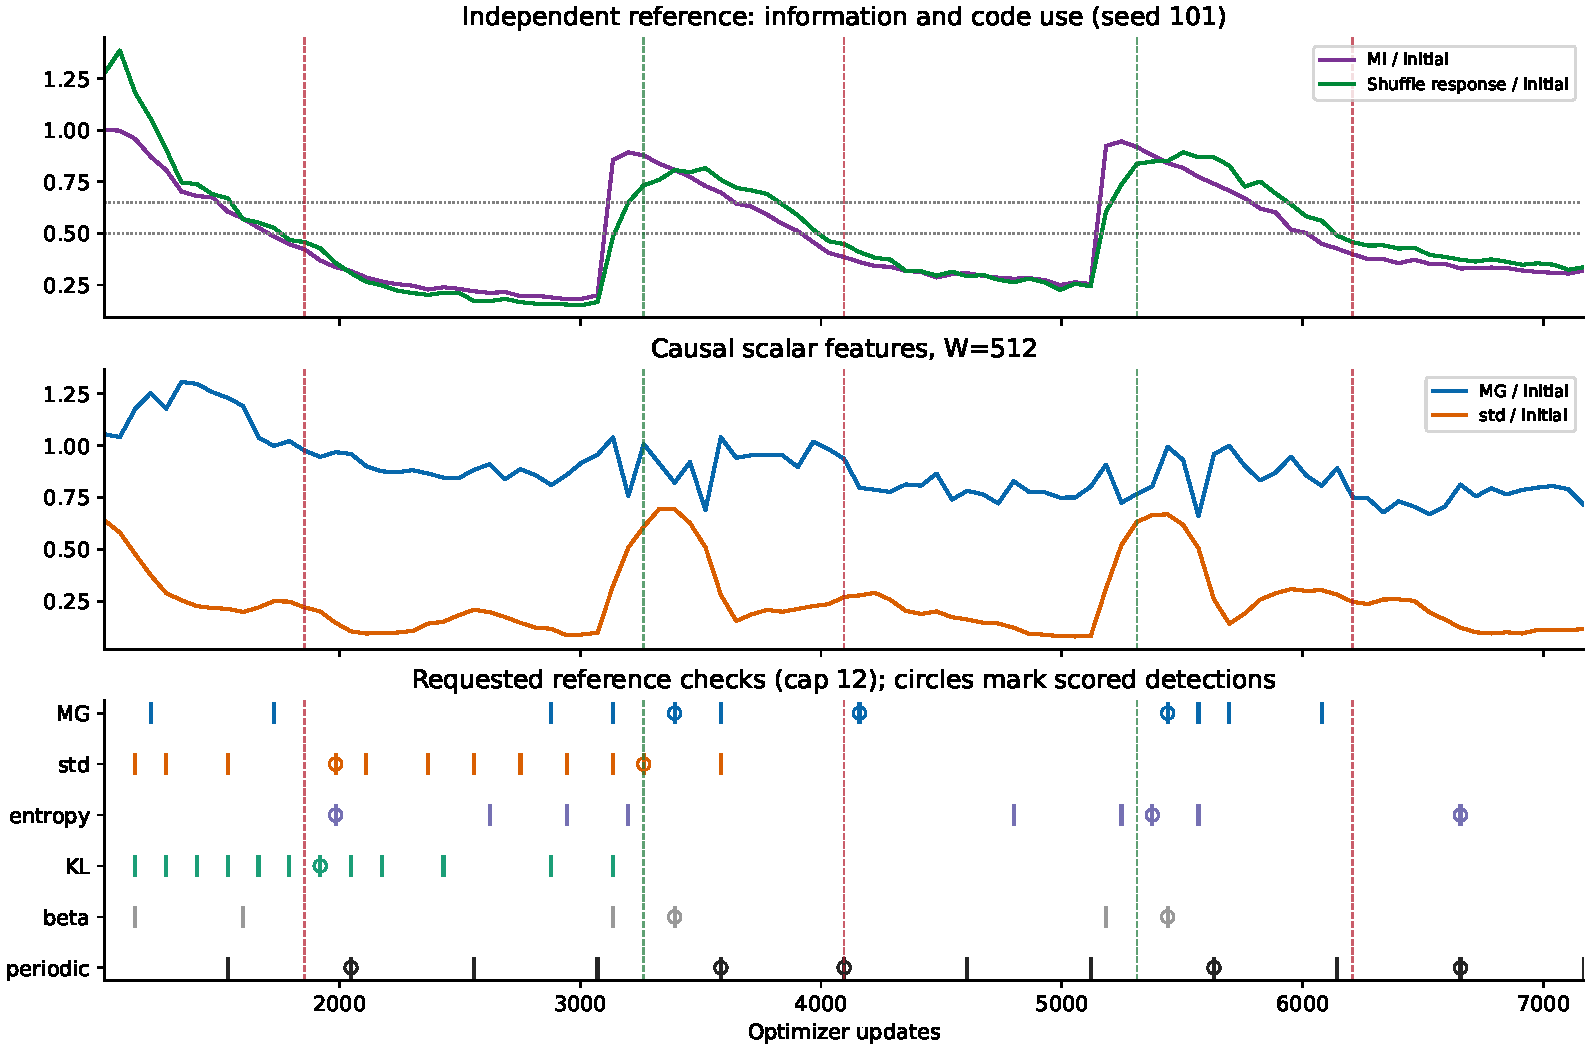
\includegraphics[width=\linewidth,height=.30\textheight,keepaspectratio]{example.pdf}\end{center}

Seed 101 выбран заранее как первый подтверждающий запуск. Сверху --- два независимых показателя, делённые на исходный уровень; в центре --- MG и отклонение loss; внизу --- запросы диагностики. Красные вертикали --- подтверждённая потеря информации, зелёные --- восстановление. Кружки отмечают зачтённые обнаружения. Последующие значения ряда при принятии решения не используются.

\textbf{Вход мониторов.} MG получает только reconstruction NLL/token на фиксированных 16 проверочных предложениях и фиксированном Gaussian noise, по одному наблюдению до каждого обновления. Окно 512, вложение 20, delay 1, 20 соседей, Theiler 39; без удаления тренда. Отклонение loss и нормированная спектральная энтропия получают то же окно. KL --- среднее последних 64 обучающих KL, уже вычисляемых в loss. Beta --- известное расписание. Встреченные численно вырожденные окна MG в подтверждающих запусках: 0.

\section*{4. Полная стоимость, включая получение входного ряда}

Операции измерены после прогрева в одном процессе, 40 чередующихся повторов на CPU: forward probe --- 7,13 мс; полная диагностика --- 209,32 мс; MG одного окна --- 12,89 мс. Torch использует 2 потока, оцениватель --- 1. Времена параллельного обучения не используются. На машине может работать другая задача, поэтому это локальная оценка стоимости компонентов, не точный benchmark изолированного сервера.

\begin{center}\small
\begin{tabularx}{\linewidth}{l>{\raggedright\arraybackslash}X>{\raggedright\arraybackslash}X>{\raggedright\arraybackslash}X>{\raggedright\arraybackslash}X}
\toprule
Способ & Получение ряда, с & Обработка + проверки, с & Всего, с & Если ряд уже записан, с \\
\midrule
MG & 51,14 & 3,54 & 54,68 & 3,54 \\
Отклонение loss & 51,14 & 2,73 & 53,86 & 2,73 \\
Спектр. энтропия & 51,14 & 2,45 & 53,59 & 2,45 \\
KL обучения & 0,00 & 2,72 & 2,72 & 2,72 \\
Расписание beta & 0,00 & 1,47 & 1,47 & 1,47 \\
Равные интервалы & 0,00 & 2,72 & 2,72 & 2,72 \\
\bottomrule\end{tabularx}\end{center}

В стоимость MG/std/entropy включены все 7168 дополнительных forward probe, 105 вычислений признака и выбранные вызовы диагностики. Последний столбец применим только когда именно этот фиксированный probe уже записывался для другой цели. Обычный KL уже входит в обучение и не требует дополнительного forward. Плотная схема: 97 диагностик, 20,30 с, все подтверждённые события обнаруживаются по построению эталона. Сокращение числа вызовов нельзя приравнивать к ускорению: нужно оплатить получение признака и учитывать пропущенные события.

Для MG без заранее записанного probe окупаемость относительно плотной схемы начинается, если один вызов независимой диагностики стоит более 606,5 мс при неизменных остальных затратах. Это расчёт порога, не экспериментальное подтверждение ускорения на более крупной модели.

\newpage

\section*{5. Все seed, перенос порога и границы результата}

\begin{center}\small
\begin{tabularx}{\linewidth}{l>{\raggedright\arraybackslash}X>{\raggedright\arraybackslash}X>{\raggedright\arraybackslash}X>{\raggedright\arraybackslash}X}
\toprule
Seed & Событий & MG: найдено / проверок & Равные интервалы: найдено / 12 & Интервалы с числом проверок MG \\
\midrule
101 & 5 & 3/11 & 5/12 & 5/11 \\
102 & 5 & 4/10 & 3/12 & 4/10 \\
103 & 4 & 3/8 & 4/12 & 4/8 \\
104 & 5 & 2/9 & 4/12 & 3/9 \\
105 & 5 & 4/12 & 5/12 & 5/12 \\
106 & 4 & 4/7 & 4/12 & 3/7 \\
107 & 4 & 2/12 & 4/12 & 4/12 \\
108 & 4 & 3/8 & 4/12 & 4/8 \\
109 & 5 & 3/8 & 5/12 & 2/8 \\
\bottomrule\end{tabularx}\end{center}

При точном совпадении числа проверок по каждому seed MG обнаруживает 28 событий, периодическая схема --- 34. Этот дополнительный периодический контроль знает итоговое число запросов, но не времена событий; это сопоставление затрат после эксперимента, не заранее выбранное число запросов. При общем лимите 12 MG лучше периодической схемы на 1 seed, равен на 1, хуже на 7.

\begin{center}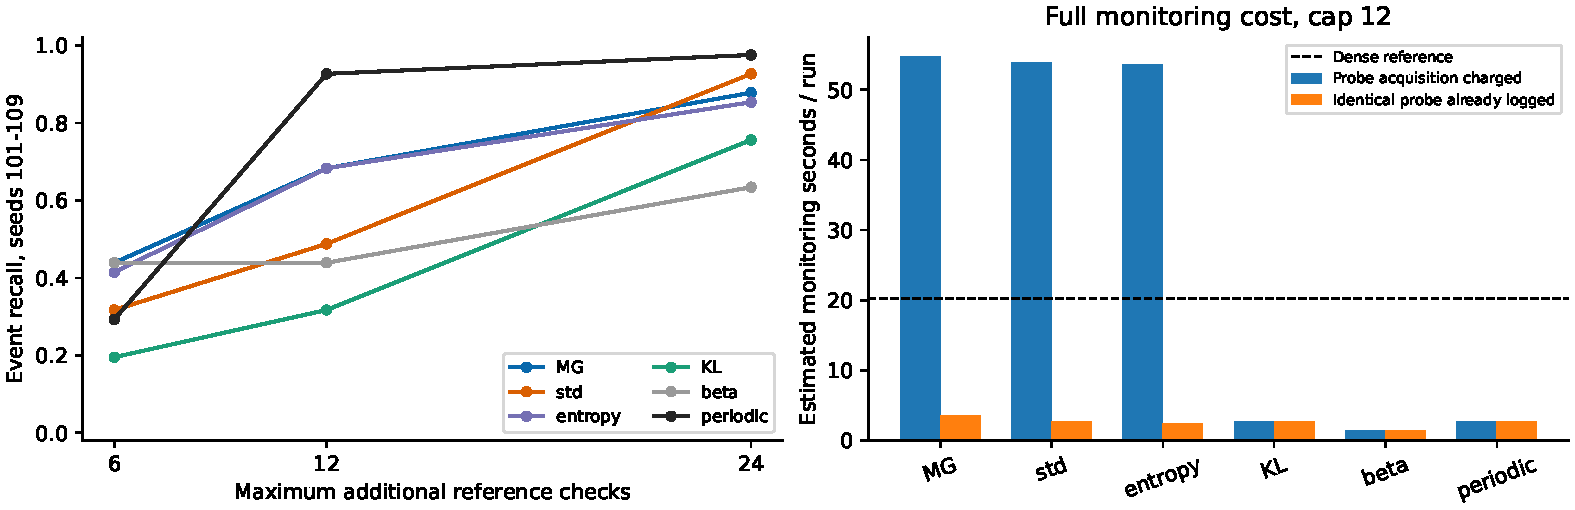
\includegraphics[width=\linewidth,height=.30\textheight,keepaspectratio]{cohort.pdf}\end{center}

Слева доля найденных событий при лимитах 6, 12 и 24; справа полная стоимость при лимите 12. Пороги каждого способа и бюджета выбраны только на пилоте 100 и затем заморожены. Средняя по seed разность recall MG минус равные интервалы при лимите 12 --- -24,4 процентного пункта; 95\% парный bootstrap по девяти seed --- [-36,7; -10,0], 20000 повторов. Окна и события внутри seed не считались независимыми выборками. Все запуски используют один корпус и probe.

\textbf{Точная политика.} На шагах 1088, 1152, ... сравниваем текущий признак с его значением при последнем запросе (изначально --- медиана пяти предшествующих окон). Запрос срабатывает, когда абсолютное значение логарифма отношения достигает порога, прошло не менее 128 шагов и бюджет не исчерпан. Пороги при лимите 12: MG: 0,20; std: 0,30; entropy: 0,50; KL: 0,15; beta: 1,50. Перебор 14 заранее заданных порогов на пилоте максимизирует число обнаружений, затем минимизирует бесполезные проверки и задержку. Для всех признаков применяется одна общая схема; это сравнение конкретных политик, а не доказательство оптимальности MG или слабости всех возможных KL-мониторов. При маленьком пороге бюджет может закончиться рано.

\textbf{Другой бюджет.} При лимите 6 MG находит 18/41, равные интервалы --- 12/41, но бесплатное расписание beta даёт 18/41. Преимущество MG над периодической схемой здесь не означает преимущества над всеми простыми альтернативами.

\textbf{Вывод для статьи.} Практическое преимущество выбранного MG-монитора в основном сравнении не подтверждено. Это отдельная проверка полезности мониторинга, а не опровержение ранее наблюдавшегося согласования MG с потерей информации. Следует учитывать обнаружения, задержку и полную стоимость одновременно. Циклы одинаковы во всех запусках, что благоприятно для периодических проверок; перенос на неизвестные расписания, другие корпуса и LLM не проверен. Точная размерность и улучшение генерации текста не оценивались.

Все логи, веса, события, решения, пилотный перебор, замороженные пороги и независимые проверки сохранены. Подробности: PROTOCOL.md и README.md. Результаты прежних парных и защищённых режимов не подменяются новой серией; их отчёты сохранены отдельно.
\end{document}